\documentclass[12pt,a4paper]{article}
\usepackage[utf8]{inputenc}
\usepackage[italian]{babel}
\usepackage{amsmath}
\usepackage{amsfonts}
\usepackage{braket}
\usepackage{amssymb}
\usepackage{graphicx}
\usepackage{hyperref}
\usepackage[left=2cm,right=2cm,top=2cm,bottom=2cm]{geometry}
\newcommand{\rem}[1]{[\emph{#1}]}

\author{Belliardo Federico}
\title{Integer Quantum Hall Effect}
\begin{document}
\maketitle

\begin{abstract}
Si presenta qui una prima teoria per spiegare l'effetto Hall quantistico intero.
\end{abstract}

\section{L'effetto Hall classico}

\begin{figure}[!htb]
\centering
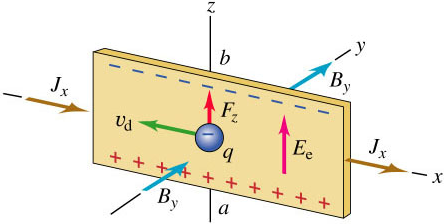
\includegraphics[scale=1.0]{immagini/classicalHall.png}
\caption{Disegno schematico dell'effetto Hall classico.\label{alpha}}
\end{figure}

Consideriamo un insieme di elettroni confinati una superficie bidimensionale su cui trasversalmente è applicato un campo magnetico. L'equazione di moto classica è:

\begin{equation}
m \frac{d \mathbf{v}}{d t} = - e \bold{E} - e \mathbf{v} \times \mathbf{B} - \frac{m \mathbf{v}}{\tau}
\end{equation}

Il coefficiente $\tau$ è il tempo di scattering e riassume qualsiasi impedimento al moto dell'elettrone (impurità, altri elettroni, ...).

Cerchiamo una soluzione stazionaria dell'equazione del moto ricordando che 
\begin{equation}
\mathbf{J} = - n e \mathbf{v}
\end{equation}

abbiamo ($\mathbf{J}$ e $\mathbf{B}$ sono trasversali):

\begin{equation}
\left(
\begin{matrix}
1 && \omega_B \tau \\
\omega_B \tau && 1\\
\end{matrix}
\right)
\mathbf{J} = \frac{e^2 n \tau}{m} \mathbf{E}
\end{equation}

\begin{equation}
\mathbf{J} = \sigma \mathbf{E}
\end{equation}

che è la legge di \emph{Ohm}, in particolare troviamo: 

\begin{equation}
\sigma = 
\frac{\sigma_{DC}}{1 + \omega_B^2 \tau^2} 
\left(
\begin{matrix} 
1 && \omega_B \tau \\
\omega_B \tau && 1\\
\end{matrix} \right)
\end{equation}
dove $\sigma_{DC} = \frac{n e^2}{m}$. Vediamo che per avere una corrente di equilibrio $I_x \neq 0$ e $ I_y = 0$ è necessario avere anche una componente del campo elettrico lungo $y$ a causa della forma non diagonale della matrice. Questo fenomeno fu scoperto da Edwin Hall nel 1879 grazie ad un esperimento stimolato da una nota di Maxwell nel suo famoso trattato. Possiamo calcolare la resistività:

\begin{equation}
\rho = \sigma ^{-1} = \frac{1}{\sigma_{DC}}
\left(
\begin{matrix}
1 && \omega_B \tau \\
- \omega_B \tau && 1 \\
\end{matrix}
\right)
\end{equation}

sostituendo nella formula di sopra otteniamo la previsione classica:

\begin{equation}
\rho_{xx} = \frac{m}{n e^2 \tau}  \quad \rho_{xy} = \frac{B}{ne}
\end{equation}

Dunque vediamo che $\rho_{xx}$ dovrebbe essere costante al variare del campo magnetico mentre $\rho_{xy}$ è previsto crescere linearmente con il campo magnetico.

 
\section{Misura dell'effetto Hall quantistico intero.}

Nel 1980 von Klitzing studiò la resistenza di Hall del gas 2D di elettroni in un MOSFET di GaAs/AlGaAs a basse temperature e alte intensità del campo magnetico. Egli trovò che le misure  di $\rho_{xy}$ e $\rho_{xx}$ si discostavano dall'aspettativa classica e mostravano una ricca struttura.

\begin{figure}[!htb]
\centering
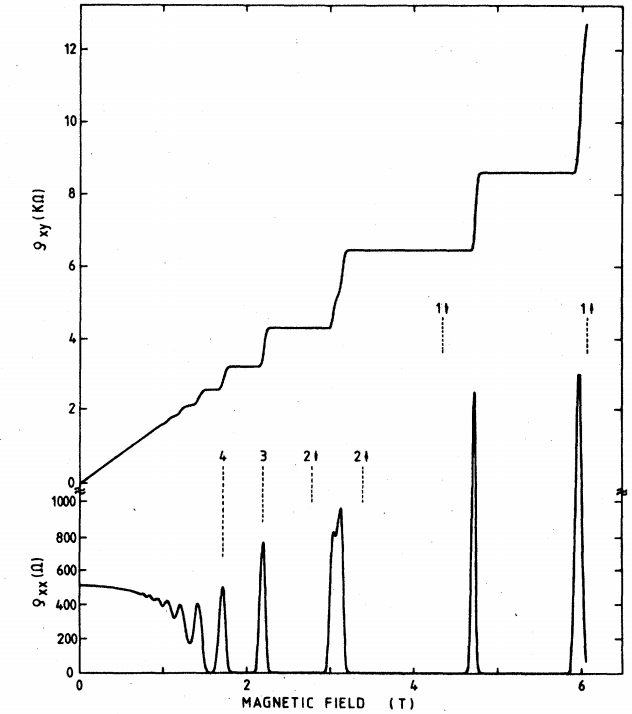
\includegraphics[scale=0.4]{immagini/integer.png}
\caption{Misure della resistività $\rho_{xy}$ e $\rho_{xx}$ di von Klitzing per le quali vinse il primio Nobel nel 1985.\label{von}}
\end{figure}

Alcune osservazioni sulle misure:

\begin{itemize}
\item La resistività è quantizzata secondo la legge: \[ \rho_{xy} = \frac{2 \pi  \hbar}{e^2} \frac{1}{\nu} \quad \nu \in \mathbb{Z} \] Questa quantizzazione non dipende da alcuna proprietà del materiale come densità di elettroni o impurezze. Per la sua natura universale questo fenomeno è usato per misure precise dell'unità di resistenza e per misurare la costante di struttura fine. 
\item Per piccoli campi magnetici l'andamento misurato è effettivamente quello classico.
\item $\rho_{xy}$ presenta una serie di \emph{plateau} con una transizione \emph{sharp} tra uno e l'altro. 
\item $\rho_{xx}$ invece è diverso da $0$ solamente durante le transizioni da un \emph{plateau} all'altro. quando ci si trova su un \emph{plateau} non c'è resistività lungitudinale.
\item Aumentando il disordine del campione (impurità) si vede che i \emph{plateau} diventano più definiti. In questo effetto il disordine svolge un ruolo costruttivo.

\item Non è mostrato nella figura ma a più alti campi magnetici iniziano ad apparire plateau a valori frazionari della resistenza. Questo fenomeno è noto come \textit{effetto Hall quantistico frazionario}.
\end{itemize}

\begin{figure}[!htb]
\centering
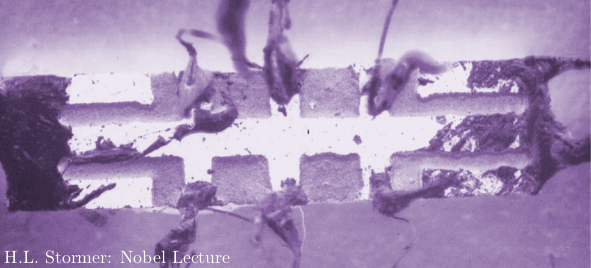
\includegraphics[scale=0.6]{immagini/real.png}
\caption{Fotografia di un campione di GaAs/AlGaAs.\label{sample}}
\end{figure}

\section{Elettroni di Bloch in campo magnetico}
Per spiegare l'IQHE si studierà un modello di elettroni non interagenti in campo magnetico trasverso  su un background periodico. Scriviamo l'Hamiltoniana di singola particella:
\begin{equation}
\mathcal{H} = \frac{(\mathbf{p} + e \mathbf{A})^2}{2m} + U(x, y)
\end{equation}

dove $U(x+a,y) = U(x, y+b) = U(x, y)$.

In ciò che segue trascureremo lo spin dell'elettrone. A livello di elettroni non interagenti l'unico effetto che avrebbe sarebbe la degenerazione di spin, ma a basse temperature e per grandi campi magnetici gli spin sono tutti allineati lungo $\mathbf{B}$ quindi non si verifica nemmeno la doppia occupazione di ogni livello perché è energeticamente sfavorita.

L'introduzione del campo magnetico rompe la simmetrica discreta dell'Hamiltoniana per traslazioni nel reticolo di Bravais diretto.

Al fine di caratterizzare gli autostati dell'Hamiltoniana introduciamo gli operatori di traslazione magnetici: 
\begin{equation}
T_{R} = \exp \left( \frac{i \mathbf{R} \cdot \left( \mathbf{p} + e \mathbf{A} \right)}{\hbar} \right)
\end{equation}
Questi dipendono dalla scelta della gauge e si vede che commutano con l'Hamiltoniana $$[T_{R}, \mathcal{H}] = 0$$
tuttavia questi operatori di traslazione non commutano tra di loro, infatti:
$$ T_{a} T_{b} = \exp \left( 2 \pi \phi \right) T_{b} T_{a} $$ dove $\phi = \left( \frac{e B}{h} \right) ab$ è il numero di flussi magnetici elementari $\frac{h}{e}$ nella cella del reticolo.
Non abbiamo quindi speranza di diagonalizzare contemporaneamente tutti gli operatori di traslazione.

Tuttavia facendo l'ipotesi che sia $\phi = \frac{p}{q}$ con $p, q$ due numeri interi (possiamo sempre sceglierli con precisione arbitraria) abbiamo la speranza di diagonalizzarne alcuni. 
Consideriamo il sottoreticolo definito dalle traslazioni 
\begin{equation}
\mathbf{R} = n(q \mathbf{a}) + m \mathbf{b}
\end{equation}
queste commutano tra di loro. 
Classificheremo dunque gli autostati con gli autovalori di $\mathcal{H}$, $T_{q \mathbf{a}}$, $T_{b}$. In particolare sarà:
$$T_{qa} \psi = \exp \left( i k_1 qa \right) \psi$$
$$T_{b} \psi = \exp \left( i k_2 b \right) \psi$$

dove $k_1$ e $k_2$ sono i quasi-impulsi magnetici. Essi possono essere ristretti nella zona di Brillouin magnetica: $$0 \leq k_1 \leq \frac{2 \pi}{qa} \quad 0 \leq k_2 \leq \frac{2 \pi}{b}$$ 

Si ricorda che per il teorema spettrale normale gli operatori hermitiani (come l'Hamiltoniana) e unitari (come le traslazioni) possono essere diagonalizzati da una base ortonormale di autovettori.\\
Dunque diagonalizzo prima $T_{qa}$ trovando una base ortonormale, i suoi autospazi sono invarianti per $T_{b}$, che posso diagonalizzare all'interno di ognuno di essi sempre con una base ortonormale. Ripeto la procedura per l'Hamiltoniana all'interno di ogni sottospazio $\bold{k}$.  Ottengo dunque un insieme ortogonale di autovettori.

Gli autostati sono quindi: 
\begin{equation}
\psi^{(\alpha)}_{\mathbf{k}} (\mathbf{x}) =  \exp \left( i \mathbf{k} \cdot \mathbf{x} \right) u^{(\alpha)}_{\mathbf{k}} (\mathbf{x})
\end{equation}
dove $\alpha$ è l'indice di banda (in generale $\alpha$ sono tutti gli altri numeri quantici che  servono per costruire lo spazio di Hilbert, nelle nostre applicazioni si tratta solamente di un numero intero che è l'indice di banda). $u$ sono delle funzione invarianti per gli operatori di traslazione magnetica.
%Come già detto gli operatori di traslazione dipendono dalla scelta della gauge. Scegliamo la gauge simmetrica e scriviamo:
%\begin{equation}
%T_{R} = \exp \left[ \frac{i \mathbf{R} \cdot \left( \mathbf{p} + e %\frac{\mathbf{x} \times \mathbf{B}}{2}  \right)}{\hbar} \right]
%\end{equation}

%deve essere: 
%\begin{equation}
%\begin{split}
%T_{qa} u^{(\alpha)}_{\mathbf{k}} (\mathbf{x}) = u^{(\alpha)}%_{\mathbf{k}} (\mathbf{x})\\
%T_{b} u^{(\alpha)}_{\mathbf{k}} (\mathbf{x}) = u^{(\alpha)}%_{\mathbf{k}} (\mathbf{x})\\
%\end{split}
%\end{equation}

%da questa, applicando le definizioni, derivano le relazioni:

%\begin{equation}
%\begin{split}
%u^{(\alpha)}_{\mathbf{k}} (x + qa, y) = \exp \left( - \frac{i \pi p y}%{b} \right)  u^{(\alpha)}_{\mathbf{k}} (x, y) \\
%u^{(\alpha)}_{\mathbf{k}} (x, y+b) = \exp \left( \frac{i \pi p x}{qa} %\right)  u^{(\alpha)}_{\mathbf{k}} (x, y)\\
%\end{split}
%\end{equation}


%La variazione totale della fase quando si percorre il bordo rettangolare chiuso della zona di Brillouin magnetica (percorso in senso orario) è invariante di gauge e vale $2 \pi p$. Pertanto se scriviamo $$ u^{(\alpha)}_{\mathbf{k}} (x, y) = |  u^{(\alpha)}_{\mathbf{k}} (x, y) | \exp \left[ i \theta_{\mathbf{k}} (\mathbf{x}) \right]$$
%abbiamo che
%\begin{equation}
%p = -\frac{1}{2 \pi} \int d \mathbf{l} \cdot \frac{\partial %\theta_{\mathbf{k}} (\mathbf{x})}{\partial \mathbf{l}}
%\end{equation}
 
%Definiamo la variazione della fase della funzione d'onda lungo un certo cammino in senso antiorario in unità di $2 \pi$ come la sua vorticosità. Sappiamo per esempio che nel caso di uno zero semplice la vorticosità in un intorno dello zero è vincolata a essere $\pm 1$. Nelle righe precedenti abbiamo ricavato che la vorticosità della funzione d'onda lungo il cammino chiuso che identifica la zona di Brillouin magnetica è vincolato è essere $-p$ indipendentemente dalla gauge scelta, questo è un primo risultato topologicamente significativo.  

\section{La conduttanza di Hall come risposta lineare}
Affronteremo pedissequamente il problema di determinare la conduttanza \emph{bulk} del gas di elettroni sfruttando la formula di Kubo per la risposta lineare. 

Consideriamo un sistema generico (anche  a molti corpi interagente) e accendiamo un campo elettrico esterno uniforme che descriviamo in  termini di $\mathbf{A}$ scegliendo $\phi = 0$, dunque $$\Delta \mathcal{H} = - \mathbf{J} \cdot \mathbf{A}$$ dove $\mathbf{J}$ è la corrente elettrica associata al sistema in esame.
%Stiamo assumendo che solamente la materia in questa situazione sia quantizzata e il campo elettrico che stimola la risposta del sistema sia abbastanza forte da potersi considerare classico.
Poiché gli esperimenti di QHE sono fatti a temperatura bassa possiamo assumere $T = 0$ e eseguire il calcolo in rappresentazione di interazione. Si suppone che il sistema cominci a evolvere sotto l'effetto dell'Hamiltoniana di interazione a partire dal ground state $\ket{0}$:
\begin{equation}
\bra{0(t)} \mathbf{J}(t) \ket{0(t)} = \bra{0} U^{-1} (t) \mathbf{J}(t) U(t) \ket{0} = \bra{0} \left( \mathbf{J}(t) + \frac{i}{\hbar} \int_{-\infty}^{t} dt' \left[\Delta H (t'), \mathbf{J}(t)\right] \right) \ket{0}
\end{equation} \label{calcolo}
Ci limitiamo a calcolare la risposta lineare perché supponiamo di eseguire misure con piccoli campi elettrici, di fatto misuriamo: $\rho_{xy} = \frac{\partial J_y}{\partial E_x} \Bigr|_{E_x = 0}$. 

Scegliamo per comodità di calcolo $\mathbf{A} = \frac{\mathbf{E}}{i \omega} \exp \left( i \omega t \right)$ dunque otteniamo:
\begin{equation}
\langle J_y(t) \rangle = \frac{1}{\hbar \omega} \int_{-\infty}^{t} dt' \bra{0} \left[ J_{x} (t'), J_{y}(t) \right] \ket{0} E_{x} e^{-i \omega t'}
\end{equation}
Abbiamo assunto che il valore di aspettazione della corrente sul ground state non interagente fosse nullo: $\bra{0} \mathbf{J} \ket{0} = 0$.

Poiché abbiamo calcolato la risposta al primo ordine immaginando di far agire la perturbazione da $-\infty$ arrivati al tempo al tempo $t$ siamo ormai in condizioni stazionarie e possiamo sfruttare l'invarianza temporale osservando che l'integrando può veramente dipendere solo da $t'' = t - t'$:

\begin{equation}
\langle J_y(t) \rangle = \frac{1}{\hbar \omega} \left( \int_{0}^{+\infty} dt'' \, e^{i \omega t''} \bra{0} \left[ J_{x} (0), J_{y}(t'') \right] \ket{0} \right) E_{x} e^{-i \omega t}
\end{equation}

otteniamo finalmente la formula di Kubo per la conduttività:

\begin{equation}
\sigma_{xy} (\omega) = \frac{1}{\hbar \omega} \int_{0}^{+\infty} dt \, e^{i \omega t} \bra{0}\left[ J_{y} (0), J_{x}(t) \right] \ket{0}
\end{equation}

Della derivazione di questa formula possono chiaramente essere messi in dubbio l'approssimazione lineare e l'ipotesi di stazionarietà.\\

Inseriamo un insieme completo di autostati dell'Hamiltoniana e scriviamo $\mathbf{J(t)} = V(t)^{-1} \mathbf{J(0)} V(t)$ dove $V(t) = \exp \left( - i \hbar \mathcal{H}_{0} \right)$. Otteniamo:

\begin{equation}
\sigma_{xy} = \frac{1}{\hbar \omega} \int_{0}^{+\infty} dt \; e^{i \omega t} \sum_{n} \left[ \bra{0} J_{y} \ket{n} \bra{n} J_{x} \ket{0} e^{i \frac{(E_n - E_0)t}{\hbar}} -
\bra{0} J_{x} \ket{n} \bra{n} J_{y} \ket{0} e^{i \frac{(E_0 - E_n)t}{\hbar}} \right]
\end{equation}


%Per assicurare la convergenza dell'integrale dobbiamo assumere che sia stata accesa adiabaticamente il che significa dopo aver cambiato variabili che dobbiamo assumere $\omega \rightarrow \omega + i0^{+}$. 
Eseguendo l'integrale temporale e ricordando che il ground state non contribuisce alla conduttività arriviamo a:

\begin{equation}
\sigma_{xy} (\omega) = - \frac{i}{\omega} \sum_{n \neq 0} \left[ \frac{\bra{0} J_{y} \ket{n} \bra{n} J_{x} \ket{0}}{\hbar \omega + E_n - E_0} - \frac{\bra{0} J_{x} \ket{n} \bra{n} J_{y} \ket{0}}{\hbar \omega + E_0 - E_n} \right]
\end{equation}

Si capisce che l'ipotesi di questa formula è che il ground state non sia degenere così che non si abbiano divergenze nel denominatore.

Ora vogliamo specificare questa formula nel caso in cui i conduttori di corrente siano $N$ elettroni indipendenti. Lo stato quantistico \emph{many-body} è dunque fattorizzabile e lo si può inserire nella formula ricavata considerando tutte le possibili occupazioni dei livelli da parte degli elettroni. 
In maniera più semplice si può argomentare che lo stato iniziale degli elettroni occupanti gli stati più bassi disponibili fino alla superficie di Fermi sarà scrivibile come:

\[
\ket{0} = \frac{A}{\sqrt{N}}\ket{\psi_1}\ket{\psi_2} ... \ket{\psi_N}
\]

Dove $A$ è l'operatore che antisimmetrizza la funzione d'onda.\\
L'operatore di evoluzione temporale si spezza e i ket dei singoli elettroni evolvono indipendentemente, abbiamo dunque:
\[
\bra{0(t)} \mathbf{J}(t) \ket{0(t)}  = \frac{1}{N}\bra{\psi_1(t)} \bra{\psi_2 (t)} ... \bra{\psi_N (t)} A^{-1} \left( \bold{J}_1 (t) + ... +  \bold{J_N} (t) \right) A \ket{\psi_1(t)} \ket{\psi_2 (t)} ... \ket{\psi_N (t)} = 
\]
\[
= \bra{\psi_1(t)} \bold{J}_1 (t) \ket{\psi_1(t)} + \bra{\psi_2(t)} \bold{J}_2 (t) \ket{\psi_2(t)} + ... + \bra{\psi_N(t)} \bold{J}_N (t)  \ket{\psi_N(t)}
\]

Infatti il valore di aspettazione su un determinante di Slater di una somma di operatori a singola particella si scrive come la somma dei valori di aspettazione dei singoli operatori su ogni possibile stato degli elettroni.

Consideriamo un elettrone che si trovi nella funzione d'onda $\ket{\psi^{(\alpha)}_{\mathbf{k}} (\mathbf{x})}$ il suo contributo alla conduttività è: 
\begin{equation}
\sigma_{xy} (\omega) = -  \frac{i}{\omega} \sum_{\beta \neq \alpha} \left[ \frac{ \bra{\psi^{(\alpha)}_{\mathbf{k}}} J_{y}  \ket{\psi^{(\beta)}_{\mathbf{k'}}} \bra{\psi^{(\beta)}_{\mathbf{k'}  }} J_{x} \ket{\psi^{(\alpha)}_{\mathbf{k}} }}{\hbar \omega + E^{\beta}(\mathbf{k'}) - E^{\alpha}(\mathbf{k})} -
 \frac{ \bra{\psi^{(\alpha)}_{\mathbf{k}} } J_{x}  \ket{\psi^{(\beta)}_{\mathbf{k'}} } \bra{\psi^{(\beta)}_{\mathbf{k'}} } J_{y} \ket{\psi^{(\alpha)}_{\mathbf{k}}}}{\hbar \omega - E^{\beta}(\mathbf{k'}) + E^{\alpha}(\mathbf{k})}
\right]
\end{equation}


In questa formula e in tutte le successive si è sottintesa la somma sugli indici di banda $\bold{k}$.
Il contributo di tutti gli elettroni si ottiene quindi sommando su $\alpha$:

\begin{equation}
\sigma_{xy} (\omega) = - \frac{i}{\omega} \sum_{\alpha, \beta \neq \alpha} \left[ \frac{ \bra{\psi^{(\alpha)}_{\mathbf{k}}} J_{y}  \ket{\psi^{(\beta)}_{\mathbf{k'}}} \bra{\psi^{(\beta)}_{\mathbf{k'}  }} J_{x} \ket{\psi^{(\alpha)}_{\mathbf{k}} }}{\hbar \omega + E^{\beta}(\mathbf{k'}) - E^{\alpha}(\mathbf{k})} -
 \frac{ \bra{\psi^{(\alpha)}_{\mathbf{k}} } J_{x}  \ket{\psi^{(\beta)}_{\mathbf{k'}} } \bra{\psi^{(\beta)}_{\mathbf{k'}} } J_{y} \ket{\psi^{(\alpha)}_{\mathbf{k}}}}{\hbar \omega - E^{\beta}(\mathbf{k'}) + E^{\alpha}(\mathbf{k})}
\right]
\end{equation}

dove $\alpha$ indica gli stati occupati e $\beta$ indica ogni altro possibile stato. La suddetta formula assumeva che il contributo alla corrente dello stato $\ket{0}$ fosse nullo, per poter dire il primo termine della formula (15) è nullo.  Questo non è vero per ogni singolo elettrone, ma è vero quando si considerano gli stati 
$\ket{\psi^{(\alpha)}_{\mathbf{k}}}$ e $\ket{\psi{(\alpha)}_{\mathbf{-k}}}$.

Sappiamo che $\mathbf{J} = \frac{e}{m} \left( \mathbf{p} + e \mathbf{A} \right) = e \mathbf{v}$, dunque abbiamo (introducendo una notazione semplificata):
\begin{equation}
\sigma_{xy} (\omega) = - \frac{i e^2}{\omega} \sum_{\alpha, \beta \neq \alpha} \left[ \frac{ \bra{\alpha}v_{y}  \ket{\beta} \bra{\beta} v_{x} \ket{\alpha}}{\hbar \omega + E^{\beta} - E^{\alpha}} -
 \frac{ \bra{\alpha} v_{x}  \ket{\beta} \bra{\beta} v_{y} \ket{\alpha}}{\hbar \omega - E^{\beta} + E^{\alpha}}
\right]
\end{equation}
Ora vogliamo considerare il caso $\omega \rightarrow 0$ che è il caso statico che ci interessa: 
\begin{equation}
\frac1{\pm\hbar\omega + E^{\alpha} - E^{\beta}} = \frac1{E^{\alpha} - E^{\beta}}\left(1 \mp \frac{\hbar\omega}{E^{\alpha} - E^{\beta}}\right) + \mathcal O(\omega^2)
\end{equation}


Scriviamo $\sigma = \sigma_1 + \sigma_2$:

\begin{equation}
\sigma^1 = \frac{-ie^2}{\omega} \sum_{\alpha,\beta \neq \alpha} \frac{\langle \alpha|v_x|\beta \rangle \langle \beta|v_y|\alpha \rangle + \langle \alpha|v_y|\beta \rangle \langle \beta|v_x|\alpha \rangle}{E^{\alpha} - E^{\beta}}
\end{equation}

\begin{equation}
\sigma^2 = -ie^2\hbar \sum_{\alpha,\beta \neq \alpha} \frac{- \langle \alpha|v_x|\beta \rangle \langle \beta|v_y|\alpha \rangle + \langle \alpha|v_y|\beta \rangle \langle \beta|v_x|\alpha \rangle}{(E^\alpha - E^\beta)^2} .
\end{equation}

Il primo termine a causa della serie geometrica nelle energie potrebbe divergere ma non lo fa, vediamolo:

\[ \langle \alpha | v_x | \beta \rangle = \langle \alpha | H_0 x - x H_0 | \beta \rangle = (E^{\alpha}-E^{\beta}) \langle \alpha | x | \beta \rangle \]

\[
\sigma^1 = \frac{-ie^2}{\omega} \sum_{\alpha,\beta \neq \alpha} \frac{(E^{\alpha}-E^{\beta})\langle \alpha|x|\beta \rangle \langle \beta|v_y|\alpha \rangle - (E^{\alpha}-E^{\beta})\langle \alpha|v_y|\beta \rangle \langle \beta|x|\alpha \rangle}{E^{\alpha} - E^{\beta}}
\]

\[
\sigma^1 = \frac{-ie^2}{\omega} \sum_{\alpha,\beta \neq \alpha} \langle \alpha|x|\beta \rangle \langle \beta|v_y|\alpha \rangle - \langle \alpha|v_y|\beta \rangle \langle \beta|x|\alpha \rangle
\]


Introduco la relazione di completezza: $\sum_{\beta \neq \alpha} |\beta \rangle\langle \beta| = 1 - |\alpha \rangle\langle \alpha|$, cioè sommo su tutti i $\beta$ diversi da $\alpha$. Rimane ancora la sommatoria il $\alpha$. Ottengo:

\[
\sigma^1 = \frac{-ie^2}{\omega} \sum_{\alpha} \left[ \langle \alpha|x\left( 1 - |\alpha\rangle \langle \alpha| \right) v_y|\alpha \rangle - \langle \alpha|v_y \left( 1 - | \alpha\rangle \langle \alpha|  \right) x|\alpha \rangle \right]
\]

\[
\sigma^1 = \frac{-ie^2}{\omega} \sum_{\alpha} \left[ \langle \alpha|xv_y - v_yx |\alpha \rangle - \langle \alpha|x | \alpha\rangle \langle \alpha|  v_y|\alpha \rangle + \langle \alpha|v_y | \alpha \rangle \langle \alpha|  x| \alpha \rangle \right]
\]

Gli operatori $x$ e $v_y$ commutano, dunque il primo termine si cancella. Il secondo anche è nullo per ogni $\alpha$.

Scriviamo dunque l'equazione ottenuta per la conduttività:

\begin{equation}
\sigma^2 = -ie^2\hbar \sum_{\alpha,\beta \neq \alpha} \frac{- \langle \alpha|v_x|\beta \rangle \langle \beta|v_y|\alpha \rangle + \langle \alpha|v_y|\beta \rangle \langle \beta|v_x|\alpha \rangle}{(E^\alpha - E^\beta)^2} .
\end{equation}

Come abbiamo detto precedentemente la somma  su $\alpha$ è fatta sugli stati occupati dagli elettroni e il significato di $\beta \neq \alpha$ è di evitare la divergenza a denominatore (non si intende $\beta$ diverso da tutti gli $\alpha$ ma solo da quello particolare che stiamo considerando nel subtotale). Osserviamo che se $\beta = u$ è uno stato occupato allora per ogni $\alpha = v$ esiste un elemento della somma in cui si scambiano $\beta = v$ e $\alpha = u$, dunque essendo la frazione antisimmetrica per scambio di $\alpha, \beta$ otteniamo l'equazione finale per la conduttività lineare:

\begin{equation}
\sigma^2 = -ie^2 \hbar \sum_{E^{\alpha} < E_{F} < E^{\beta}} \frac{- \langle \alpha |v_x|\beta \rangle \langle \beta |v_y|\alpha \rangle + \langle \alpha |v_y|\beta \rangle \langle \beta |v_x|\alpha \rangle}{(E^\alpha - E^\beta)^2} .
\end{equation}

Stiamo ora supponendo di trovarci a cavallo tra due bande, in particolare è una nostra ipotesi che sia vera una sorta di struttura a bande per il sistema.

Dove abbiamo indicato con $E_{F}$ l'energia di Fermi e la somma è fatta per $\alpha$ che corre sugli stati al di sotto di essa e $\beta$ sugli stati al di sopra. Scriviamo l'equazione di Schrödinger come: $$ \mathcal{H} (\mathbf{k}) u^{(\alpha)}_{\mathbf{k}} (\mathbf{x}) = E^{\alpha} (\mathbf{k}) u^{(\alpha)}_{\mathbf{k}} (\mathbf{x})$$ dove 
\begin{equation}
\mathcal{H} (\mathbf{k}) = \frac{(\mathbf{p} + \hbar \mathbf{k} + e \mathbf{A})^2}{2m} + U(x, y) 
\end{equation}
Ricordiamo che in tutte le formule l'indice di banda $\mathbf{k}$ è sempre sottinteso.

Dato $\mathbf{v} = \frac{-i \hbar \mathbf{\nabla} + e \mathbf{A}}{m}$, abbiamo che la velocità commuta con le traslazioni magnetiche, quindi essa non può cambiare $\mathbf{k}$, ovviamente l'Hamiltoniana non commuta con la velocità.\\
In particolare gli operatori di traslazione magnetici commutano separatamente con la velocità e con il potenziale periodico $U(x, y)$. Vediamo che lo stato $\bold{v}  \psi_{\mathbf{k}}^{\alpha}$ appartiene allo stesso autospazio caratterizzato dall'autovalore $\bold{k}$ quindi esso potrà avere prodotto scalare non nullo solamente con i vettori all'interno dello stesso autospazio:

\[
T_{qa} \left( \bold{v}  \psi_{\mathbf{k}}^{\alpha} \right) = \bold{v} \left( T_{qa}  \psi_{\mathbf{k}}^{\alpha} \right) = e^{i k_1 q a} \bold{v}  \psi_{\mathbf{k}}^{\alpha}
\]

Possiamo dunque scrivere:

\[
\bra{\alpha} v_{x} \ket{\beta} = \delta_{\mathbf{k}, \mathbf{k'}} \int_{0}^{qa} dx \int_{0}^{b} dy  \quad \psi_{\mathbf{k}}^{\alpha *} \mathbf{v} \psi_{\mathbf{k'}}^{\beta} = \delta_{\mathbf{k}, \mathbf{k'}} \int_{0}^{qa} dx \int_{0}^{b} dy  \quad e^{-i \bold{k} \cdot \bold{x}} u_{\mathbf{k}}^{\alpha *} \frac{\bold{p} + e \bold{A}}{m} \left( e^{i \bold{k'} \cdot \bold{x}} u_{\mathbf{k'}}^{\beta} \right)= 
\]

\[
=\delta_{\mathbf{k}, \mathbf{k'}} \int_{0}^{qa} dx \int_{0}^{b} dy  \quad e^{-i \bold{k} \cdot \bold{x}} e^{i \bold{k'} \cdot \bold{x}} u_{\mathbf{k}}^{\alpha *} \frac{\bold{p} + \hbar \bold{k'} + e \bold{A}}{m}  u_{\mathbf{k'}}^{\beta}= \delta_{\mathbf{k}, \mathbf{k'}} \frac{1}{\hbar}\int_{0}^{qa} dx \int_{0}^{b} dy  \quad u_{\mathbf{k}}^{\alpha *} \frac{\partial \mathcal{H}}{\partial \bold{k}}  u_{\mathbf{k'}}^{\beta}
\]


Poiché il valore di aspettazione è non nullo solo tra stati con stesso $\mathbf{k}$ possiamo limitare l'integrale ad una cella magnetica dello spazio reale, perché nelle altre entrambe le funzioni di cui si calcola il prodotto scalare prendono la stessa fase che si cancella nel valore di aspettazione. Le funzioni $u(\bold{x})$ normalizzate sulla cella magnetica del reticolo di Bravais.

Poiché $\alpha$ e $\beta$ hanno lo stesso $\mathbf{k}$ possiamo scrivere:
\begin{equation}
\begin{split}
\bra{\alpha} v_{x} \ket{\beta} = \frac{1}{\hbar} \left \langle {\alpha} \bigg{|} \frac{\partial \mathcal{H}}{\partial k_x} \bigg{|} \beta \right \rangle \\
\bra{\alpha} v_{y} \ket{\beta} = \frac{1}{\hbar}  \left \langle \alpha \bigg{|} \frac{\partial \mathcal{H}}{\partial k_y} \bigg{|} \beta \right \rangle\\
\end{split}
\end{equation}

inoltre:
\begin{equation}
\left \langle u^\alpha \bigg{|} \frac{\partial \mathcal{H}}{\partial k_y} \bigg{|} {u^\beta} \right \rangle = (E^{\beta} - E^{\alpha}) \left \langle u^\alpha \bigg{|}\frac{\partial u^{\beta}}{\partial k_{j}} \right \rangle = - (E^{\beta} - E^{\alpha})\left \langle \frac{\partial u ^{\alpha}}{\partial k_{j}} \bigg{|} u^\beta \right \rangle
\end{equation}

Arriviamo dunque a scrivere:
\begin{equation}
\sigma_{xy} = \frac{i e^2}{\hbar} \sum_{E^{\alpha} < E_{F} < E^{\beta}} \int \frac{d^2 k}{(2 \pi)^2} \left[\braket{\partial_y u^{\alpha} | u^{\beta}} \braket{u^{\beta}|\partial_x u^{\alpha}} - \braket{\partial_x u^{\alpha}|u^{\beta}}\braket{u^{\beta}|\partial_y u^{\alpha}}\right]
\end{equation}

Dove abbiamo reintrodotto esplicitamente la somma sugli stati a $\mathbf{k}$ diverso.

Ora usiamo il fatto che $$\sum_{E^{\alpha} < E_F}  \ket{\alpha} \bra{\alpha} + \sum_{E_{F} < E^{\beta}} \ket{\beta}\bra{\beta} = 1$$ 

Portiamo la somma sugli stati non occupati all'interno dell'integrale e otteniamo:

\[
\sigma_{xy} = \frac{i e^2}{\hbar} \sum_{\alpha} \int \frac{d^2 k}{(2 \pi)^2} \left[\braket{\partial_y u^{\alpha} | \partial_x u^{\alpha}} - \braket{\partial_x u^{\alpha} | \partial_y u^{\alpha}} + \sum_{\alpha'} \braket{\partial_y u^{\alpha} | \alpha' } \braket{\alpha' | \partial_x u^{\alpha}} - \braket{\partial_x u^{\alpha} | u^{\alpha'}} \braket{u^{\alpha'} | \partial_y u^{\alpha}} \right]
\]

l'ultimo pezzo si scrive:

\[
\sum_{\alpha', \alpha} \left[ \braket{\partial_y u^{\alpha} | u^{\alpha'} } \braket{u^{\alpha'} | \partial_x u^{\alpha}} - \braket{\partial_x u^{\alpha} | u^{\alpha'}} \braket{u^{\alpha'} | \partial_y u^{\alpha}} \right]
\]

Abbiamo visto precedentemente che:

\[
\braket{u^{\beta}|\partial u^{\alpha}} = - \braket{\partial u^{\beta}| u^{\alpha}}
\]

quando $\beta \neq \alpha$, questo segue dal fatto che funzioni $u_{\bold{k}}^{\alpha}$ e $u_{\bold{k}}^{\beta}$, a fisso $\bold{k}$ sono ortogonali, ciò segue dall'ortogonalità delle funzioni d'onda $\psi_{\bold{k}}^{\alpha}$ e dal fatto che la fase si cancella nel prodotto scalare. Sostituendo solamente nel primo dei due prodotti scalari moltiplicati:

\[
\sum_{\alpha', \alpha} \left[ - \braket{u^{\alpha} | \partial_y u^{\alpha'} } \braket{u^{\alpha'} |\partial_x  u^{\alpha}} + \braket{u^{\alpha} |\partial_x u^{\alpha'}} \braket{u^{\alpha'} | \partial_y u^{\alpha}} \right]
\]

Dunque abbiamo che la sommatoria è simmetrica nei due indici $\alpha$ e $\alpha'$ mentre l'oggetto all'interno è antisimmetrico, dunque l'intera somma è nulla.

\begin{equation}
\sigma_{xy} = \frac{i e^2}{\hbar} \sum_{\alpha} \int \frac{d^2 k}{(2 \pi)^2} \left[\braket{\partial_y u^{\alpha} | \partial_x u^{\alpha}} - \braket{\partial_x u^{\alpha} | \partial_y u^{\alpha}}\right]
\end{equation}

In questa formula abbiamo sempre supposto di potere fare una scelta della fase in modo che le $u^{\alpha}$ fossero sempre derivabili in $\bold{k}$. Se questo non è sempre vero il significato della formula per la conduttività è di definire la $\emph{field strenght}$ in regioni aperte in cui è definibile con continuità e senza singolarità ai bordi.
In ogni caso trascurando i $\bold{k}$ su cui non si può definire con continuità la fase costituisce un errore trascurabile essi sono infatti comunque insiemi di misura nulla nello spazio dei $\bold{k}$

\section{Invariante TKNN}
Arrivati a questo punto mostreremo che la conduttività trasversa è quantizzata per motivi topologici. Consideriamo la zona di Brilloiun parametrizzata dai due quasimpulsi $k_1$ e $k_2$, se identifichiamo i lati opposti essa diventa topologicamente un toro $\mathbf{T}^2$. 

Consideriamo la 2-forma definita sul toro:

\[\mathcal{F}^{\alpha} = -i \braket{\partial_y u^{\alpha} | \partial_x u^{\alpha}} +i \braket{\partial_x u^{\alpha} | \partial_y u^{\alpha}} dk_1 \wedge dk_2 \]

%NON SONO SICURISSIMO CHE SIA DEFINITO TUTTO ANCHE SUL PUNTO DI INIZIO DELLE COORDINATE

Sempre supponendo che la componente che vogliamo associare alla forma sia definibile con continuità su tutto il toro $\mathbf{T}^2$ vediamo che questa è una buona definizione di $\mathcal{F}^{\alpha}$ su tutta la varietà infatti giunti agli estremi delle coordinate è possibile semplicemente prolungarle oltre $\frac{2 \pi}{qa}$ e sovrapponendo quindi una \emph{patch} in cui le coordinate nuove sono semplicemente le traslate di quelle vecchie. Pertanto le 1-forme di base sono le stesse (il cambio di base è l'identità) così come è la stessa la componente che si vuole assegnare alla 2-forma. Ricordiamo che per definizione $u_{\bold{k}}$ sono uguali a meno di traslazioni di $\bold{k}$ di $\frac{2 \pi}{qa}$ o $\frac{2 \pi}{b}$. Dunque la definizione della 2-forma data nello stesso punto in coordinate diverse è corretta, perché le due definizioni coincidono. Riassumiamo: se la componente $-i \braket{\partial_y u^{\alpha} | \partial_x u^{\alpha}} +i \braket{\partial_x u^{\alpha} | \partial_y u^{\alpha}}$ è ben definita su tutta la varietà è possibile definire una 2-forma su tutta la varietà scegliendo le coordinate $\bold{k}$ o loro prolungamenti.\newline

%Lo sviluppo del toro su un piano permette di identificare le coordinate $k_i$ con le coordinate cartesiane sul piano. Vediamo quindi che le 1-forme associate alle coordinate sono ben definite in maniera continua anche quando raggiungiamo l'estremo delle coordinate $\bold{k}$ perché esse sono solamente le 1-forme associate alle coordinate cartesiane che sono un campo di 1-forme costanti quindi in particolare continue. Essendo anche le funzioni $u_{\bold{k}}$ definite in maniera continua agli estremi delle coordinate al forma $\mathcal{F}$ è ben definita su tutto il toro. In altre parole possiamo scegliere nuove coordinate $\bold{k}$ traslate dove le vecchie finiscono e nella regione di sovrapposizione le due definizioni di $\mathcal{F}$ coincidono. I cambi di coordinate che servono per ricoprire tutto il toro sono solamente traslazioni di $\bold{k}$ e quindi le 1-forme $dk_i$ definite in due \emph{patch} diverse coincidono (la matrice di cambio base è l'identità).

La definizione di integrale di una $n$-forma u una $n$-varietà è:

\[ \int_{\Sigma} \omega = \int_{\phi(\Sigma)} \phi^{*} \omega\]

dove $\phi: \Sigma \rightarrow \mathbb{R}^n$ è la funzione coordinate sulla varietà. 

Introduciamo una 1-forma così definita:

\begin{equation}
\mathcal{A}^{\alpha} = -i \bra{u^{\alpha}_{\mathbf{k}}} \partial_{k_1} \ket{u^{\alpha}_{\bold{k}}} dk_1 -i \bra{u^{\alpha}_{\mathbf{k}}} \partial_{k_2} \ket{u^{\alpha}_{\bold{k}}} dk_2
\end{equation}

Essa assomiglia alla connessione di Berry $U(1)$ tuttavia è concettualmente differente perché la vera connessione di Berry agisce sullo spazio dei parametri, mentre questa 1-forma vive sullo spazio degli stati. Calcoliamo la \emph{field strength} associata ad $\mathcal{A}_i$:

\begin{equation}
\mathcal{F}^{\alpha}_{xy} = \frac{\partial \mathcal{A}^{\alpha}_{x}}{\partial k_{y}}-\frac{\partial \mathcal{A}^{\alpha}_{y}}{\partial k_{x}} = -i \braket{\partial_{y} u^{\alpha}| \partial_{x} u^{\alpha}} + i  \braket{\partial_{x} u^{\alpha}| \partial_{y} u^{\alpha}}
\end{equation}

Possiamo dire che dove è definita la forma $\mathcal{A}$ vale $\mathcal{F} = d \mathcal{A}$. Notiamo che stiamo correttamente integrando una 2-forma su una 2-superficie.
Supponiamo ora che l'energia di Fermi si trovi tra una banda e l'altra così che le bande occupate siano tutte piene e l'integrale sullo spazio degli stati sia completo, siamo arrivati a:

\begin{equation}
\sigma_{xy} = -\frac{e^2}{2 \pi \hbar} \sum_{\alpha} \int_{\mathbf{T}^2} \mathcal{F}^{\alpha} dS = -\frac{e^2}{h} \sum_{\alpha} \mathcal{C}_{\alpha}
\end{equation}

L'integrale della \emph{field strength} sulla superficie del toro è noto nella teoria dell'effetto Hall quantistico come invariante TKNN, dal nome dei fisici che per primi lo hanno identificato in questo contesto (D. J. Thouless, M. Kohmoto, M. P. Nightingale e M. den Nijs). Nella matematica è noto come primo numero di Chern, esso è sempre un numero intero.

Notiamo che abbiamo una 1-forma (e quindi un'integrale sulla zona di Brillouin magnetica) diverso per ogni banda occupata del sistema. Osserviamo che abbiamo scritto la somma sullo spazio degli stati come un integrale considerando dunque gli stati come continui nel vettore d'onda. Questa è una buona approssimazione nel limite termodinamico.
Variando il campo è possibile cambiare il numero di stati in ogni banda in modo analogo a quanto succede per i livelli di Landau quindi si può cambiare il numero di bande riempite.

\section{Quantizzazione topologica}
Nelle sezioni precedenti abbiamo assunto di poter derivare impunemente le funzioni d'onda $u$ nell'indice di banda $\bold{k}$, ora analizzeremo meglio questa ipotesi. Sappiamo che le funzioni d'onda sono definite a meno di una fase globale:

\begin{equation}
u(\bold{k}) \rightarrow e^{i f(\bold{k})} u(\bold{k})
\end{equation}

Questo causa una ridefinizione del potenziale vettore (se la funzione $f(\bold{k})$ è \emph{smooth}):

\begin{equation}
\mathcal{A}_i \rightarrow \mathcal{A}_i + \nabla f(\bold{k})
\end{equation}

Perché siano ben definite la connessione e la sua curvatura è necessario che le funzioni d'onda $u(\bold{k})$ siano derivabili in $\bold{k}$. Il fenomeno significativo è che non è detto sia possibile scegliere una fase globale (una gauge) che renda \emph{smooth} le funzioni $u(\bold{k})$ su tutta la varietà. Il significo dell'invariante TKNN è di definire e integrale la \emph{field strength} sulle regioni in cui è possibile farlo separatamente e trascurare le loro frontiere (che saranno comunque un insieme di misura nulla).

Notiamo che se fosse possibile definire globalmente la connessione $\mathcal{A}$ e la sua derivata esterna allora per il teorema di Stokes il numero di Chern sarebbe nullo essendo il bordo del toro $\partial \mathbf{T}^2 = 0$.

La scelta delle regioni in cui è bene definita la connessione dipende fortemente dalle funzioni $u(\bold{k})$. Supponiamo che sia possibile prendere due zone $H_{I}$ e $H_{II}$ (vedi figura \ref{topos}) in cui sono definite le  $u(\bold{k})$ in maniera \emph{smooth} allora avrò un \emph{phase mismatch} dato da una funzione $\chi (\bold{k})$ su una corona del bordo tra le due zone. Se il \emph{phase mismatch} è una funzione continua sappiamo come sono legate tra loro le connessioni definite nelle due regioni, dunque:

\begin{equation}
\int_{\mathbf{T}^2} \mathcal{F} dS = \int_{H_{I}} \mathcal{F_{I}} dS + \int_{H_{II}} \mathcal{F_{II}} dS
\end{equation}

Ricordiamo che l'integrale TKNN è stato definito sule regioni aperte della zona di Brilloiun in cui era possibile definire la \emph{field strength}.

Applico il teorema di Stokes separatamente:

\begin{equation}
\int_{H_{I}} \mathcal{A_{I}} dS + \int_{H_{II}} \mathcal{A_{II}} dS = \int_{\partial H} \mathcal{A_{I}} \cdot d \bold{l} - \int_{\partial H} \mathcal{A_{II}} \cdot d \bold{l} = \int_{\partial H} \nabla \chi (\bold{k}) \cdot d \bold{l} = 2 \pi n 
\end{equation}

Abbiamo indicato con $\partial H$ il bordo delle due regioni del toro. Il cambio di segno occorre perché l'orientazione indotta sul bordo dalle due sottovarietà $H_{I}$ e $H_{II}$ è opposta.

La funzione $\chi (\bold{k})$ essendo per ipotesi ben definita e liscia ha come integrale su una linea chiusa un multiplo intero si $2 \pi$. 
Nella figura \ref{topos} è mostrata la fase per una componente $\braket{x_0|u_{\bold{k}}}$ della funzione d'onda. Essa è rappresentata da una freccia (il cui angolo va appunto da $0$ a $2 \pi$). Nel disegno la connessione non è scelta con continuità nella regione $H_I$.

Nelle applicazioni alla fisica dello stato solido le discontinuità si possono sempre ridurre a punti isolati. Pertanto è sempre possibile spostarle in un disco del toro  mediante un opportuna scelta della gauge per operare poi una ``chirurgia'' che sostituisca questo disco a uno in cui non vi sono singolarità (perché sono state spostate nella regione esterna).

In generale vale:
\begin{figure}[!htb]
\centering
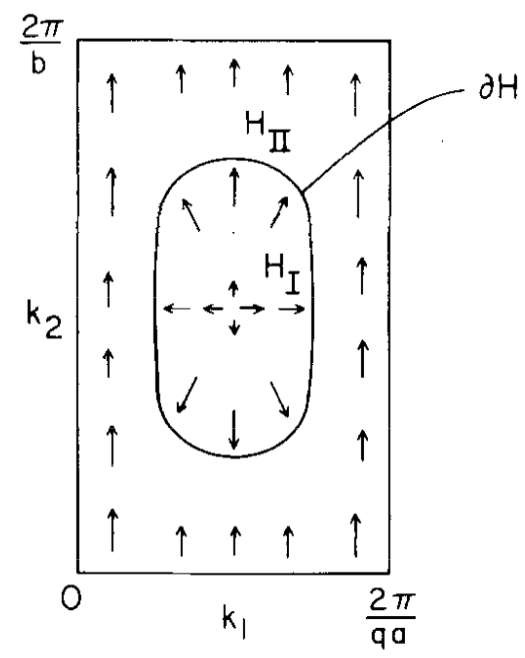
\includegraphics[scale=0.6]{immagini/magnetic.png}
\caption{Scelte della fase nella zona di Brilloiun\label{topos}}
\end{figure}

$\bold{Teorema:}$ L'integrale della 2-forma $\mathcal{F}^{\alpha}_{xy} = -i \braket{\partial_{y} u^{\alpha}| \partial_{x} u^{\alpha}} + i  \braket{\partial_{x} u^{\alpha}| \partial_{y} u^{\alpha}}$ sulla superficie di una varietà compatta, senza bordo e orientabile è quantizzato.

E' difficile dare una dimostrazione nel nostro caso senza ricorrere a strumenti di topologia algebrica o senza conoscere la forma delle funzioni d'onda $u(\bold{k})$ e mostrando esplicitamente le opportune scelte delle gauge nelle varie regioni del dominio che realizzano la liscezza.
Possiamo aspettarci che l'impossibilità di definire $u_{\bold{k}}$ su tutta la zona di Brilloiun sia dovuta alla presenza di  ``vorticosità'' nella fase di $u(\bold{k})$ per certi valori di $\bold{x}$.

La derivazione di $\sigma_{xy}$ è valida quando l'energia di Fermi si trova tra due bande, in questa situazione ci aspettiamo che il sistema si comporti da isolante in effetti mostriamo la conduttività longitudinale è nulla. Sappiamo infatti che:
$$\sigma_{xx} = \frac{\rho_{xx}}{\rho_{xx}^2 + \rho_{xy}^2} $$ e visto che $\rho_{xy}$ è non nullo otteniamo: 
\begin{equation}
\rho_{xx} = 0 \rightarrow \sigma_{xx} = 0
\end{equation}

E' possibile mostrare che sia $\sigma_{xy}$ che $\rho_{xy}$ si annullano nel limite di campi magnetici piccoli perché si annullano i numeri di Chern delle bande. A piccoli $\bold{B}$, $\rho_{xx}$ è diversa da 0 e $\sigma_{xy} = 0 \rightarrow \rho_{xy} = 0$

%Quello che ho scritto sotto è sbagliato
%Si vorrebbe anche trovare ragione del fatto che a campi magnetici piccoli ottengo per $\sigma_{xy}$ sostanzialmente la previsione classica e nel limite di campo nullo si annulla. Consideriamo il potenziale periodico che genera il reticolo come una piccola perturbazione sul campo magnetico. Ci aspettiamo che i livelli di Landau si allarghino poiché viene rotta la loro degenerazione. Al diminuire del campo magnetico un numero crescente di bande scende sotto l'energia di Fermi che rimane costante. Infatti la spaziatura tra gli infiniti livelli di Landau che si generano in 2D diminuisce al diminuire del campo magnetico. Dunque nella conduttività trasversa dobbiamo sommare tutti i numeri di Chern delle bande che stanno sotto la sfera di Fermi e che quindi contribuiscono. La conduttività tende dunque a diventare infinita e la resistività nulla. Questa rappresentazione non funziona quando il campo magnetico diventa troppo piccolo così che non si possa più vedere il reticolo come piccola perturbazione.

%\begin{figure}[!htb]
%\centering
%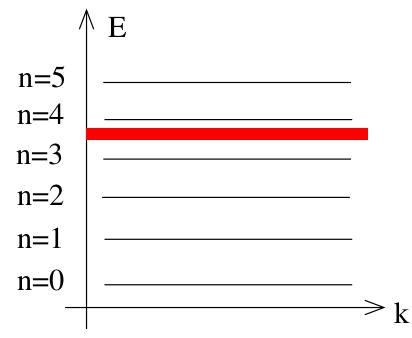
\includegraphics[scale=0.4]{immagini/landau.png}
%\caption{Livelli di Landau con l'energia di Fermi disegnata in rosso.%\label{landau}}
%\end{figure}

Si possono calcolare le funzioni d'onda e gli integrali di superficie scegliendo il potenziale $U(x, y)$ più semplice possibile a patto che sia connesso con continuità a quello vero. Una variazione continua dei parametri del problema infatti non può causare un cambiamento della quantità quantizzata: questo è il significato di invariante topologico.
\section{Conclusioni}
L'ipotesi che il flusso sia una frazione è di fatto immateriale, possiamo assumere che la funzione $\sigma_{xy}$ abbia al più un numero finito di discontinuità al variare del campo magnetico associate a un qualche fenomeno fisico che accade nel campione, dunque $\sigma_{xy}(\mathbf{B})$ è costante a tratti e i \emph{plateau} sono spaziati di $\frac{2 \pi \hbar}{e^2}$ come misurato sperimentalmente. Poiché $\rho_{xx} = 0$ abbiamo $\rho_{xy} = \frac{e^2}{2 \pi \hbar} \frac{1}{\nu}$.  Possiamo aspettarci che la descrizione data venga meno quando il livello di Fermi attraversa una banda, in questa situazione la conduttività $\sigma_{xy}$ cambia in maniera \emph{sharp} mentre $\rho_{xx}$ presenta degli \emph{spikes}.  

Presentiamo una lista (incompleta) delle direzioni in cui si potrebbe proseguire lo studio del QHE:

\begin{itemize}
\item Ruolo del disordine, stati localizzati e percolazioni: la teoria proposta non permette di descrivere le transizioni da un \emph{plateu} all'altro. Il fatto che esse diventino può \emph{sharp} all'aumentare del disordine del campione fa pensare che siano associate alla localizzazione di Anderson. Osserviamo che questo modello non è affatto robusto rispetto al disordine perché si basa sull'assunzione che esista la zona di Brillouin e questo è vero solo per potenziali rigorosamente  periodici. Quando l'energia di Fermi attraversa una banda il sistema diventa conduttore e $\rho_{xy} \neq 0 \rightarrow \sigma_{xy} \neq 0$. Fenomeni alla localizzazione e alle percolazioni rendono più \emph{sharp} questa transizione.
Esiste un argomento di Thouless che assume un'Hamiltoniana con un potenziale generico e elettroni interagenti. Si impongono generiche condizioni al bordo e si calcola la conduttività di \emph{bulk}. Nell'ipotesi che questa non dipenda dalle condizoni al bordo possiamo mediare, dunque integrare sullo spazio delle condizioni al bordo trovando nuovamente il numero di Chern.
\item \emph{Chiral edge modes}: sui bordi del materiale in cui si ha QHE si propagano modi chirali che trasportano corrente. Nella nostra teoria abbiamo trattato solamente la conduttività di \emph{bulk} trascurando quanto succede ai bordi. Si ritiene che negli esperimenti la corrente sia trasportata sia dal \emph{bulk} che dai modi \emph{edge}.
\item Argomento di Laughlin: sfruttando il concetto di flusso spettrale si può approcciare il QHE nell'ipotesi di alcune topologie particolari per il campione. 
\item Fractional Quantum Hall Effect: a campi magnetici più elevati si osservano dei multipli frazionari della conduttanza fondamentale, questi sono stati spiegati da Laughlin studiando l'interazione tra gli elettroni, che nella nostra trattazione è stata completamente trascurata.

\end{itemize}

%Possiamo dire qualcosa sul segno del numer di chern??

%TODO
%Si può ricavare \sigma_{xx} = 0 dalla formula di Kubo? Sembra dare infinto??


%Possiamo vedere per completezza che $\rho_{xx} = 0$ dalla formula di Kubo infatti il secondo termine della formula di cubo per la conduttanza longitudinale $\sigma^{2}_{xx}$ è nullo identicamente, mentre il primo $\sigma^{1}_{xx}$ diverge per $\omega \rightarrow 0$ dunque (per $\sigma_{xy} \neq 0$) la resistività statica si annulla. Ricordiamo che nelle manipolazioni che involvono la conducibilità e la resistività che questi sono tensori. 

%Rubustezza rispetto al disordine? putroppo questo modello non ne da molta perché si basa sull'ipotesi di potenziale periodico se si perde questa ipotesi non è più valida questa quantizzazione.\\

%Con questa  teoria finché l'energia di Fermi si trova in un gap spiego perché vi è il \emph{plauteau}, infatti la conduttività non può variare in modo continuo al variare dei parametri cioè al variare della connessione perché deve essere un intero. In sostanza una piccola variazione della field strengh dovuta ad un cambiamento del campo magnetico finché sono valide queste ipotesi non può cambiare la conduttanza. In altre parole posso vedere $\sigma_{x,y} = f(\mathbf{B})$ con $B$ variabile continua ma $f(\mathbf{B})$ non può essere una variabile continua.\\

%Quando è che si ha il salto da un plateau all'altro? quando non valgono più le ipotesi cioè l'energia di Fermi attraversa una banda.\\


%Non ha senso veramente assumere che il campo magnetico dia un flusso frazionario. Mi rompe la'rgomento che mi genera i plateau.

%Due osservazioni. Finché verifichiamo le ipotesi della derivazione possiamo anche variare con continuità 

%Perché mi limito sempre a usare la formula perturbativa linearizzata? Assumo di fare misure con campi elettrici piccoli e correnti piccole!

%Discutere i problemi di questo modello (è difficile generalizzare al caso di disordine)

%Mettere anche argomento di Thouless che si generalizza al caso di disordine e di elettroni interagenti (sempre per la conduttività nel bulk). E' possibile supporre che la conduttività non dipenda da condizioni al bordo?

%Piccola e veloce analisi degli stati di edge chirali. 
 

%[Accennare al pumping argument e al flusso spettrale?]

%Accennare alla percolation transizion e al ruolo del disordine

%Accennare al fractional quantum hall effect

%\section{Problemi e cose da aggiugere}
%Correggere gli errori in cui dico perché non si ha $\sigma_{xy}$ per un normale cristallo la mia spiegazione non è corretta-> qual é la spiegazione allora? Non lo so e non ho tempo di approfondire.
%Durante tutta la discussione ho sempre confuso ho sempre confuso l zona di Brillouin magnetica con il reticolo reale. Correggere questo errore. E spiegare come il numero di Chern sia legato agli zeri nella zona di Brilloiun e come si possa far vedere usando il teorema di Stokes che è intero. Tutto sta nel poter fare o meno una scelta continua della fase $\chi(k_1, k_2)$ della funzione d'onda. 
%Noi scriviamo la relazione per la conduttività assumendo di poter derivare sempre la fase, cioè ne assumiamo implicitamente la possibilità di poter sempre derivare la fase. Non provare a fare derivate di trasformazioni di gauge che sono discontinue, perché non so come si definiscono le distribuzioni sulle varietà. Semplicemente cosa ci dice la formula della conduttività ricavata?
%Abbiamo introdotto le derivate perché abbiamo sempre assunto di poter derivare la fase.
%Possiamo pensare di di ridurre l'integrale alle regioni aperte dello spazio dei parametri dove la fase è bene definita con continuità. Nella formula 26 non compare la necessità di derivare rispetto agli impulsi ma sono rispetto alle coordinate reali. In questa formula tolgo un insieme di misura nulla di stati nello spazio dei $\bold{k}$ per poter fare l'integrale.
%Vedi discussione di kohomoto! Nelle regioni in cui la fase è ben definita e continua allora anche la connessione di berry è be definita e continua. Dunque posso applicare il teorema di Stokes e concludere come conclude kohomoto.
%Dovrei discutere meglio il fatto che si possa scegliere con continuità la fase se non ho gli 0!
%E che i bordi sono veramente identificati! 
%Se costruiamo dei cerchietti attorno agli 0 e fuori da essi facciamo scorrere la fase con continuità e in maniera irrotazionale come mostra Kohomoto allor per determinare il numero di Chern è sufficiente sommare gli indici della della particolare sezione scelta sul toro. Ricordati che sceglier un punto reale $x_0, y_0$ equivale a scegliere una sezione sul toro. Questo vale anche se ho più zeri quindi posso calcolare l'indice di chern a partire dagli indici degli zeri.
%Perché dovrebbe venire banale nel caso in cui non ho campo magnetico?
%Tutte le dimostrazioni che abbiamo dato funzionano, non come quella con l'olonomia che propone baez. Questa dimostrazione funziona in generale per le 2-superfici che sono sostanzialmente tori connesi con spazi proiettivi (per gli spazi proiettivi è meno intuitivo) ma è comunque vero. 
%E' intuitivo che queste costruzioni possano essere generalizzare a una varietà generica. in particolare il fatto di poter scegliere con continuità fase della funzione d'onda dove lei non si annulla. Quanto è falsa/non banale questa cosa??
%Perché la fase è banale se non ho campo magnetico??

%Di fatto la fase della funzioni d'onda $u(k1, k2)$ è una cosa totalmente arbitraria la posso anche scegliere in maniera in maniera discontinua e senza alcuna logica. La cosa topologica è che ho dei vincoli a sceglierla in maniera in maniera continua. Come posso mostrare che la cosa funziona in generale?

%Dire due parole sui fibrati principali.

%Analogia con il monopolo di Dirac??

%La quantizzazione essendo topologica è robusta anche al cambio del potenziale periodico, posso scegliere quindi il potenziale che più mi aggrada.

%La cosa interessante di questa quantizzazione è che  mascroscopica e lontana 6 o 7 ordini di grandezza dalla ragione reale per cui succede (la meccanica quantistica delle particell nel reticolo). Le cose che crediamo quantizzate a livello microscopico lo potrebbero essere in maniera topologicamente resistente a causa  di una teoria sottostante più fondamentale.

%E' diventato lo standard della reistenza e della misura della struttura fine.
%Da questo effetto nascono gli studi sugli isolanti topologici, i semimetalli di wayl, il grafene.
%Si pensa che gli anioni del fractiona quantum hall effect (molto più delicato) possano essere usati per effettuare una topological quantum computation robusta. 
%L'effetto che abbiamo descritto è il precursore di tutti gli studi sulla topologia della fisica della materia.



%Vediamo meglio la definizione della connessione:

%\begin{equation}
%\mathcal{A}_i = -i \bra{u_{\mathbf{k}}} \partial_{k_i} \ket{u_{\bold{k}}} = \int |u(\bold{k})|^2 %\frac{\partial \theta ( \bold{k} ) }{\partial \bold{k}} -i \int  |u(\bold{k})| \frac{\partial |%u(\bold{k})|}{\partial \bold{k}}
%\end{equation}

%Perché sia ben definita è necessario che siano derivabili sia il modulo che la fase delle funzioni d'onda nel parametro $\bold{k}$.


%Vediamo perché può succedere che non si riesca a assegnare con continuità una fase globale continua a tutti gli stati. Supponiamo di assegnare una fase alle funzioni d'onda $u_{\bold{k}}$ imponendo che $\braket{x_0|u_{\bold{k}}}$ sia reale. (La possiamo assegnare con continuità in una regione in cui $\braket{x_0|u_{\bold{k}}}$ non si annulla.)

%Questo è vero poiché $u(\bold{k})$ è continua in $\bold{k}$ come numero complesso in quanto soluzione dell'equazione parametrica: \footnote{Questa affermazione potrebbe essere giustificata meglio.}

%\begin{equation}
%\frac{(\mathbf{p} + \hbar \mathbf{k} + e \mathbf{A})^2}{2m} u(\bold{x}, \bold{k}) + U(x, y) %u(\bold{x}, \bold{k}) = E u(\bold{x}, \bold{k})
%\end{equation}

%Se $u(\bold{k})$ è continua in $\bold{k}$ è $|u(\bold{k})| \neq 0$ significa che le fasi sono %vicine per $\bold{k}$ vicini quindi posso annullare la fase di $\braket{x_0|u_{\bold{k}}}$ in %maniera continua. 

%TODO:Non è chiarissimo perché dovrei poter anche avere la continuità della fase per x diversi da x_0. 


%Suddividiamo la zona di Brillouin in zone in cui sia possibile assegnare con continuità la fase globale e in cui sia quindi bene definita la connessione.

%Dovrei mostrare che può succedere veramente e che tutto si trivializza se non ho campo magnetico.
%Può non essere veramente semplice mostrare in astratto che in questa situazione non posso fare questa scelta globale continua. Tuttavia è sufficiete quello che dico per mostrare che il chern number è un intero. In particolare non collego il discorso agli 0 della funzione d'oda. ma dico semplicemete che il problema potrebbe venire da vortici o divegenze della fase globale a fissato x0 che non sono eliminabili. IL modulo deve essere derivabile er richiesta fisica.
%Non faccio il collegamento con il teorema degli indici.


%dire che la fase globale è smooth non significa niente. L'effrmazione correntta è può essere impossibile scegliere la fase globale in modo da rendere la funzione u smooth e poterci fare le derivate. questa è la frase corretta. 

%\begin{equation}
%\mathbf{J} = \mathbf{J_1} + \mathbf{J_2} + \mathbf{J_1} + ... + \mathbf{J_N}
%\end{equation}

%Dove $\mathbf{J_i}$ è la corrente associata all'i-esimo elettrone.
%Per scrivere le funzioni d'onda dobbiamo considerare N stati dell'Hamiltoniana di singola particella da riempiere con gli elettroni (e antisimmetrizzare). Indicati con $u_i$ gli stati scelti abbiamo che:

%\begin{equation}
%\ket{n} = P(\ket{u_1} \ket{u_2}  \ket{u_3}  \ket{u_4}  \ket{u_5}  ... \ket{u_N} )
%\end{equation}

%dove $P$ è il proiettore sulla potenza esterna dello spazio di Hilbert di N elettroni $\Lambda^{2} H^{ \otimes N}$.

%Considero un elemento di matrice come $\bra{0} J_{y} \ket{n}$ questo è:

%$$\bra{0} J_{y} \ket{n} = \frac{1}{N} \left(\sum_{\pi} \bra{u_1^{G}(\pi(1))} \bra{u_2^{G}(\pi(2))} ... \bra{u_N^{G}(\pi(N))} \right) \left( J^{1}_{y} + J^{2}_{y} + ... + J^{N}_{y} \right)$$
%$$\left(\sum_{\pi} \ket{u_1(\pi(1))} \ket{u_2(\pi(2))} ... \ket{u_N(\pi(N))} \right)
%$$

%Nella formula sopra $\ket{u_i^{G}}$ sono gli stati del ground state, mentre $\ket{u_i}$ sono stati generici.

%Abbiamo visto prima che la fase $\theta(\bold{k}, \bold{x})$ deve essere continua per ogni scelta $di $\bold{x}$.

%Dove ho degli $0$ di $\braket{x_0|u_{\bold{k}}}$ l'assegnamento della fase in $\bold{x_0}$ non funziona più. Anche trovando un valore di $\bold{x}$ in cui le funzioni d'onda non si annullano al variare di $\bold{k}$ la fase di $u(\bold{x}, \bold{k})$ può presentare delle discontinuità al variare di $\bold{x}$.

%In generale possiamo suddividere lo spazio in zone in cui la fase delle funzioni d'onda è bene definita e continua in $\bold{k}$ al variare di $\bold{x}$.

%Essendo l'unica libertà che abbiamo sulla scelta della fase globale nella zona d....


%Per trattare queste regioni è necessario scegliere un nuovo punto $x_1$ in cui $\braket{x_0|u_{\bold{k}}}$ non si non si annulla e ripetere il ragionamento.



%Ricordiamo che una forma chiusa è una per cui vale $d \omega = 0$. $\mathcal{F}$ delle sezioni precedenti può essere scritto localmente come $\mathcal{F} = d \mathcal{A}$, con $\mathcal{A}$ una 1-forma.
%Se possiamo scrivere globalmente $\mathcal{F} = d \mathcal{A}$ su tutto il toro allora la forma $\mathcal{F}$ si dice esatta. E' noto che ostruzioni topologiche del dominio impediscono a una forma chiusa di essere sempre esatta.\newline
%Se abbiamo $\mathcal{F}$ forma esatta possiamo applicare il teorema di Stokes:
%\begin{equation}
%\int_{\mathbf{T}^2} \mathcal{F} dS = \int_{\partial \mathbf{T}^2} \mathcal{A} dl = 0
%\end{equation}
%poiché $\partial \mathbf{T}^2 = 0$, in quanto il toro è una varietà compatta senza bordo.

%Per avere una conduttanza trasversa non banale è necessario che non sia possibile definire le connessioni $\mathcal{A^{\alpha}}$ in maniera continua globalmente su tutta la varietà. Questo è garantito proprio dalla fase di origine magnetiche le funzioni $u^{\alpha}(\mathbf{k})$ prendono quando vengono traslate da un estremo all'altro della zona di Brillouin. Se queste fasi fossero nulle (come in assenza di campo magnetico) allora $\mathcal{A}$ sarebbe ben definita ai \emph{due} bordi identificati della zona di Brilloiun dunque il teorema di Stokes implicherebbe $\sigma_{xy} = 0$. In effetti in un cristallo non ci aspettiamo correnti trasverse al campo elettrico locale.\\

%TODO
%Motivare in maniera più convincente il fatto che stiamo integrando la curvatura di una connessione, cioè mostriamo che A è una connessione e motivano l'applicazione delle formule di Chern.

%Ora mostriamo attraverso un argomento generale che il numero di Chern è intero.\\
%Consideriamo una varietà compatta $\Sigma$ senza bordo ($\partial \Sigma=0$) e una forma chiusa $\mathcal{F}$. Dimostriamo che:
%\begin{equation}
%\mathcal{C} = \frac{i}{2 \pi} \int_{\Sigma} \mathcal{F} dS \in \mathbb{Z}
%\end{equation}

%Considero un punto di $\Sigma$ e un suo intorno $U(P)$, scelgo un cammino $\gamma \in U(P)$. Osservo che $\partial (\Sigma / U(P)) = \gamma$ e $\partial U(P) = \gamma$. L'orientazione dell'intorno $U(P)$ pensato come sottovarietà induce un'orientazione sul bordo $\gamma$. Scelgo l'orientazione delle due sottovarietà $U(P)$ e $\partial (\Sigma / U(P))$ verso l'esterno del toro e questo induce orientazioni opposte sui bordi. Nel seguito chiameremo $U(P) = \Sigma_1$ e $\Sigma / U(P) = \Sigma_2$.\\
%Considero un ricoprimento ${K_{i}}$ di $\Sigma_1$ tale che in ogni intorno sia possibile definire in maniera continua la connessione $\mathcal{A}$ con $d \mathcal{F}=\mathcal{A}$. 

%Decompongo il laccio $\gamma$ in un prodotto di lacci $\gamma_i \in K_i$ tali che $\prod_{i} \gamma_i = \gamma$.\\
%Indichiamo con $H(\gamma, \mathcal{A})$ l'olonomia della connessione $\mathcal{A} $ calcolata lungo il percorso chiuso $\gamma$, cioè:
%\begin{equation}
%H(\gamma, \mathcal{A}) = \exp \left( - \int_{\gamma} \mathcal{A} dl \right)
%\end{equation}

%L'olonomia di una connessione è invariante per trasformazioni di gauge: $\mathcal{A} \rightarrow \mathcal{A} + d \Lambda$
%Posso affermare che il prodotto delle olonomie è l'olonomia del commino prodotto. Questa affermazione è falsa e non posso concludere la dimostrazione.

%Si può anche mostrare che il numero TNKK è legato alla vorticità totale della funzione d'onda nella zona di Brillouin, cioè al numero totale di $0$ contati con la loro vorticità ($\pm 1$).\newline

%TODO: Dire che che il primo numero di Chern è l'unico invariante topologico che abbiamo in questo sistema.

%La teoria proposta non permette di descrivere queste transizioni. Il fatto che esse diventino può marcate all'aumentare del disordine del campione fa pensare che siano associate alla localizzazione di Anderson.\\
%Osserviamo che questo modello non è affatto robusto rispetto al disordine perché si basa sull'assunzione che esista la zona di Brillouin e questo è vero solo per potenziali rigorosamente  periodici.

\section{Bibliografia}
\begin{enumerate}
\item K. von Klitzing, G. Dorda, M. Pepper, \emph{New Method for High-Accuracy Determination of the Fine-Structure Constant Based on Quantized Hall Resistance}, Phys. Rev. Lett. 45, 494
(1980)
\item D. Thouless, M. Kohmoto, M. Nightingale, M. den Nijs, \emph{Quantized Hall Conductance in a Two-Dimensional Periodic Potential}, Phys. Rev. Lett. 49, 405, (1982)
\item R. Laughlin, \emph{Quantized Hall conductivity in two dimensions}, Phys. Rev. B 23, 5632 (1981)
\item M. V. Berry, \emph{Quantal phase factors accompanying adiabatic changes}, Proc. R. Soc. London Ser. A 392, 45 (1984)
\item M. Kohmoto, \emph{Topological Invariant and the Quantization of the Hall Conductance}, Annals of Physics, 160:343–354, 1985
\item T. Fukui, Y. Hatsugai, H. Suzuki, \emph{Chern Numbers in Discretized
Brillouin Zone: Efficient Method of Computing (Spin) Hall Conductances}, Journal of the Physical Society of Japan, 74(6):1674–1677, 2005
\item D. Tong, \emph{ The Quantum Hall Effect}, TIFR Infosys Lectures, DAMPT Cambridge, 2016
\end{enumerate}


\end{document}